\section{问题一：基础传播模型与多声道积分}

\subsection{单声道测量原理解释}

设声波沿长度为 $L$、与管道轴线夹角为 $\theta$ 的声道传播，流体声速为 $c$，管道轴向平均流速为 $v$。顺流和逆流传播时间可表示为
\begin{equation}
t_+ = \frac{L}{c + v\cos\theta}, \qquad
t_- = \frac{L}{c - v\cos\theta}.
\end{equation}
两式相减并整理，可得声道方向上的流速估计：
\begin{equation}
v = \frac{L}{2\cos\theta}\left(\frac{1}{t_+}-\frac{1}{t_-}\right).
\label{eq:single_velocity}
\end{equation}
若第 $i$ 个窗口持续时间为 $T_i$，等效管道截面积为 $A$，则单声道窗口体积估计为
\begin{equation}
\hat V_i = A T_i v_i.
\label{eq:single_volume}
\end{equation}
该模型结构清晰，参数物理含义明确，但它只代表单条声道上的线平均速度信息，而体积流量取决于整个圆截面的速度积分\cite{Sakhavi2022GeneralizedProfile}。因此，当截面速度剖面不均匀时，单声道速度未必等于截面平均速度。

\subsection{五声道加权积分与基础方法比较}

一条声道只覆盖截面的局部信息。为了接近截面真实平均流速，需要把不同高度处的观测按照其代表区域进行组合。声道位置、剖面识别方式以及积分权重都会影响最终的重构精度\cite{Qin2016ProfileIdentification,XiangMultipathIntegration}。还有论文提出广义速度剖面或修正因子降低固定权重对特定流型的依赖\cite{Sakhavi2022GeneralizedProfile,Gryshanova2023CorrectionFactor}。对窗口 $i$，记五条等效声道观测为 $c_{i0},\ldots,c_{i4}$，相应权重为 $w_0,\ldots,w_4$，则平均速度代理量写成
\begin{equation}
\bar v_i = \sum_{j=0}^{4} w_j c_{ij},
\end{equation}
窗口体积估计为
\begin{equation}
\hat V_i = A T_i \bar v_i.
\end{equation}
声道权重反映了各声道所代表的截面区域面积贡献或数值积分节点权重。中心声道通常对中心区域速度贡献更敏感，边缘声道可补充靠近管壁区域的速度信息。

需要说明的是，附件中的 \texttt{chord0}--\texttt{chord4} 已经由题设声道映射整理为等效声道观测量。本文在式中将 $c_{ij}$ 作为等效速度观测使用；若直接从原始传播时间或原始声道量计算，则还需通过附件给出的映射和几何系数先换算为同一量纲的等效速度代理。

附件给出的五声道位置和固定权重见表~\ref{tab:integration_weights}。Phys6 是题设提供的工程积分基线；OWICS 与 Gauss-Jacobi 在附件中的权重数值一致，统计时合并为一组先验。Lagrange 通过插值重构剖面后再积分，因而提高了两侧边缘声道的权重。等权法不区分声道代表面积和截面位置，在非均匀剖面下通常误差较大。

\begin{table}[H]
\centering
\caption{五声道位置与固定积分权重}
\label{tab:integration_weights}
\small
\begin{tabular}{lccccc}
\toprule
声道 & 归一化高度 & Phys6 & OWICS & Lagrange & 等权 \\
\midrule
chord0 & 0.7274 & 0.209874 & 0.221205 & 0.266260 & 0.200000 \\
chord1 & 0.2662 & 0.153223 & 0.112176 & 0.096121 & 0.200000 \\
chord2 & 0.0000 & 0.266827 & 0.333238 & 0.275238 & 0.200000 \\
chord3 & -0.2662 & 0.153223 & 0.112176 & 0.096121 & 0.200000 \\
chord4 & -0.7274 & 0.209874 & 0.221205 & 0.266260 & 0.200000 \\
\bottomrule
\end{tabular}
\end{table}

表~\ref{tab:baseline_mae} 汇总了四种基础积分量的窗口误差。Phys6 与 Lagrange 的 MAE 很接近，均明显低于 OWICS 和等权积分。两者的优势并不完全相同：Lagrange 的平均偏差更接近零，Phys6 则具有较小的最大绝对误差。因此，后续补偿实验将 Phys6 与 Lagrange 保留为候选物理基准。基础积分方法的比较如图~\ref{fig:mae_compare} 所示。

\begin{table}[H]
\centering
\caption{基础积分方法窗口误差比较}
\label{tab:baseline_mae}
\begin{tabular}{lccc}
\toprule
方法 & MAE(\%) & ME(\%) & 最大绝对误差(\%) \\
\midrule
Phys6 & 0.180653 & -0.136424 & 0.495146 \\
OWICS & 0.506237 & 0.506237 & 1.000727 \\
Lagrange & 0.183613 & -0.007930 & 0.644012 \\
Equal Weight & 0.637292 & 0.637292 & 1.083603 \\
\bottomrule
\end{tabular}
\end{table}

\begin{figure}[!htbp]
  \centering
  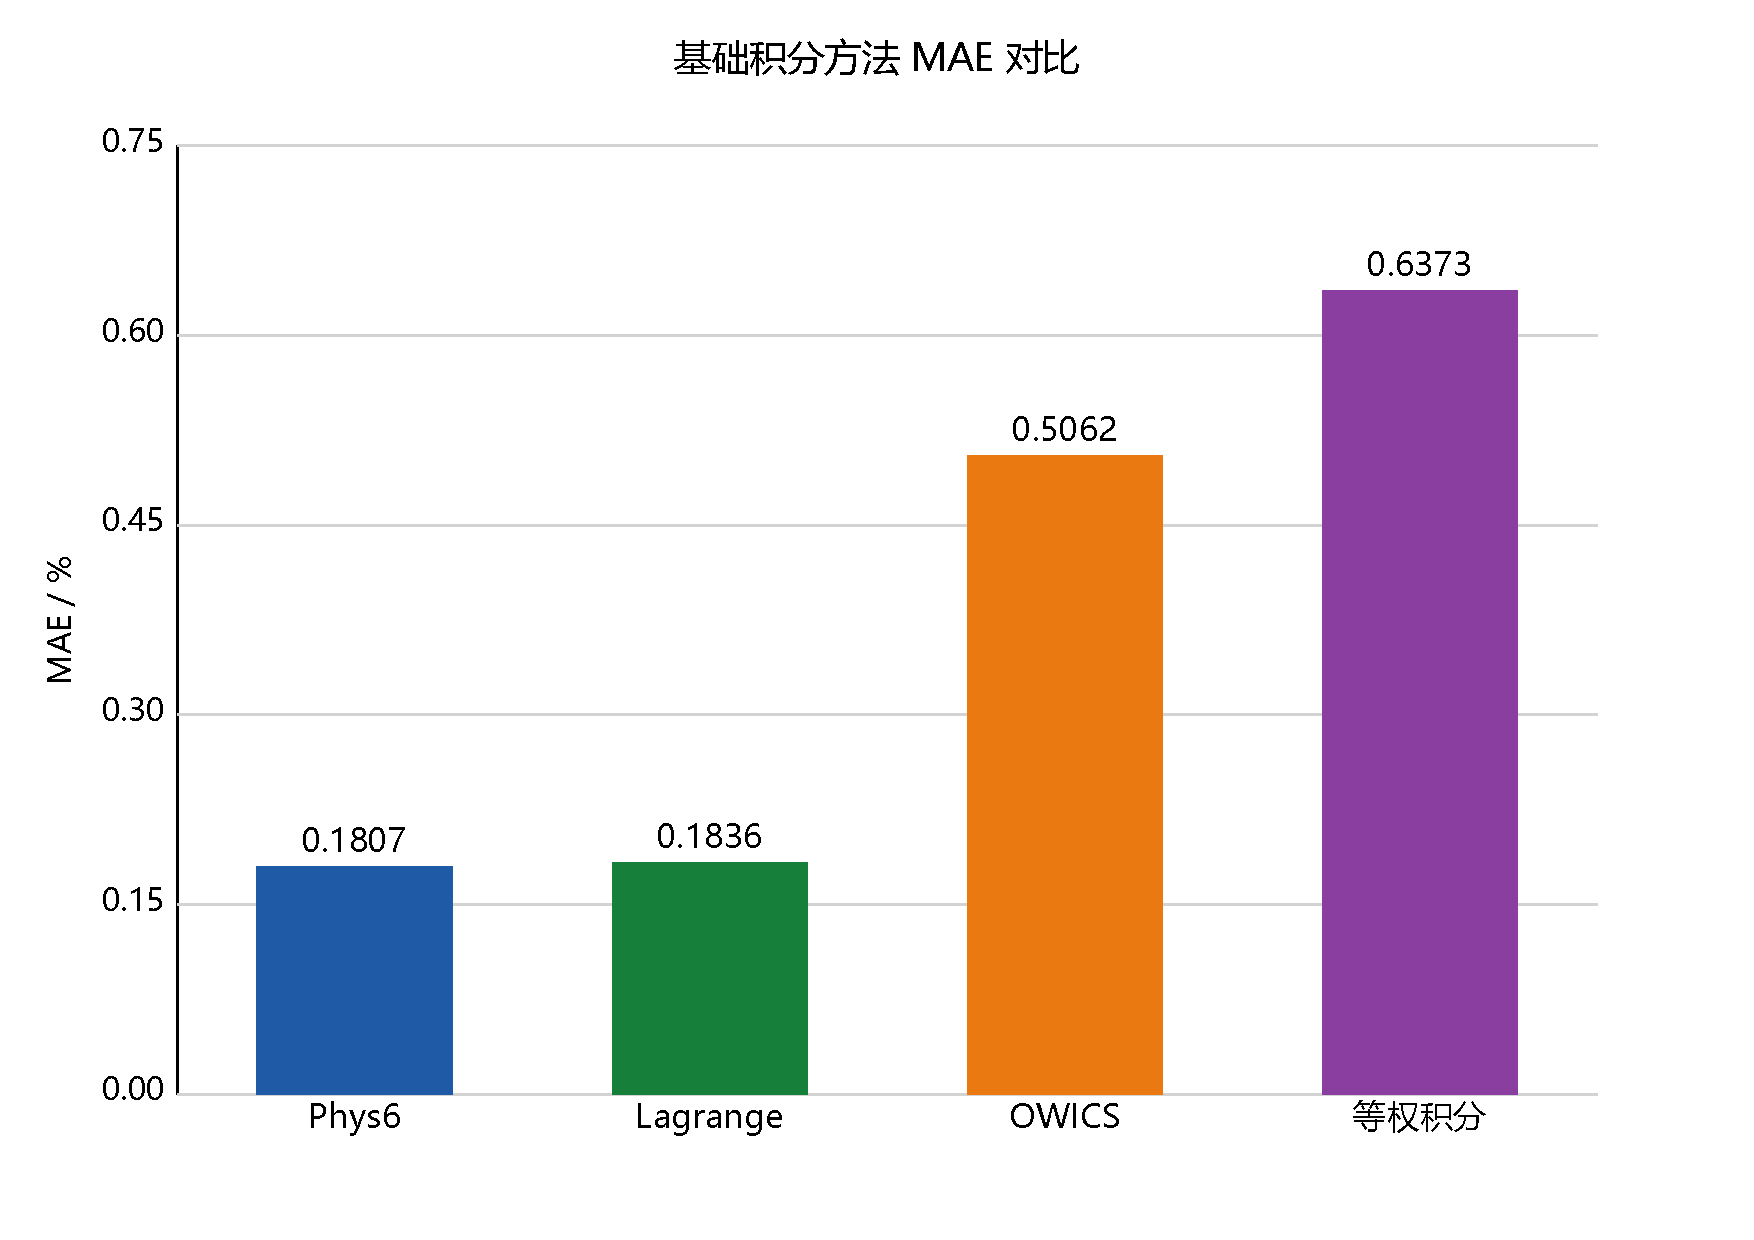
\includegraphics[width=0.88\textwidth]{../figures/fig_model_mae_comparison.pdf}
  \caption{基础积分方法 MAE 对比}
  \label{fig:mae_compare}
\end{figure}

进一步按流量点观察，如图~\ref{fig:integration_flow_mae} 所示，Phys6 和 Lagrange 在多数流量点上保持较低 MAE，而 OWICS 与等权法在部分流量段误差明显放大。这说明固定权重积分虽然能提供稳定的物理主尺度，但仍会随流量点和剖面形态发生系统偏差。

\begin{figure}[!htbp]
  \centering
  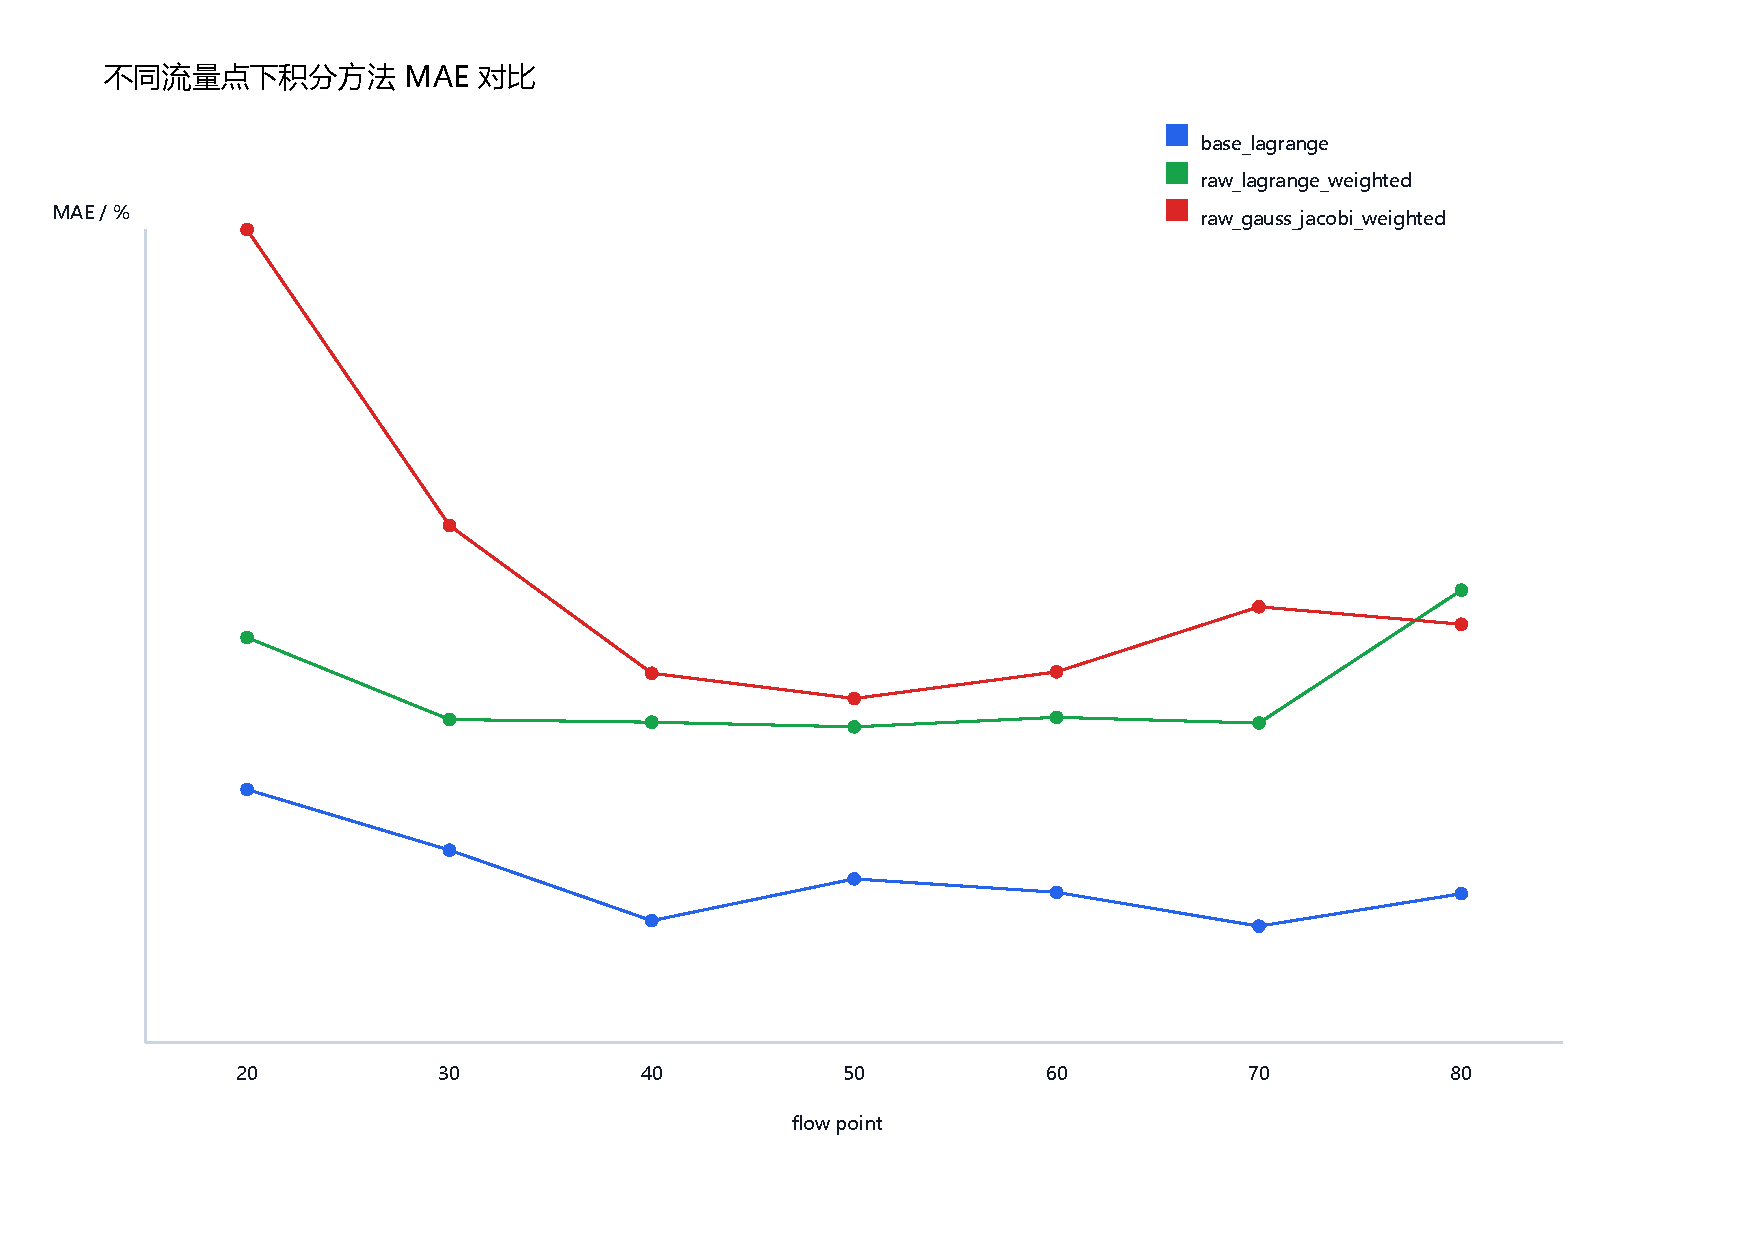
\includegraphics[width=0.88\textwidth]{../figures/fig_integration_flow_mae.pdf}
  \caption{不同流量点下基础积分方法 MAE 对比}
  \label{fig:integration_flow_mae}
\end{figure}

按工况拆分后，四种方法的表现见表~\ref{tab:baseline_condition_mae}。OWICS/Gauss--Jacobi 先验在 D0 正常工况下最优，但在 D1--D8 扰流下误差明显增加；Phys6 和 Lagrange 在扰流样本上更稳定。这说明固定积分权重与其假设的速度剖面有关，正常剖面上的最优权重不一定适合畸变剖面。

\begin{table}[H]
\centering
\caption{基础积分方法在不同工况下的 MAE（\%）}
\label{tab:baseline_condition_mae}
\begin{tabular}{lcc}
\toprule
方法 & D0 无扰流 & D1--D8 扰流 \\
\midrule
Phys6 & 0.388727 & 0.166688 \\
Lagrange & 0.523550 & 0.160799 \\
OWICS/Gauss--Jacobi & 0.226394 & 0.525019 \\
Equal Weight & 0.414760 & 0.652227 \\
\bottomrule
\end{tabular}
\end{table}
